\documentclass[11pt]{article}
\usepackage{graphicx}
\usepackage{float}
\usepackage{amsmath}
\usepackage[margin=1in]{geometry}

% report.tex sits in the project root; figures live in the question folders
\graphicspath{{q1/}{q2/}{q3/}{q4/}{q5/}}

\title{CSCI-B 657 Computer Vision -- Project 1 Report}
\author{Syed Haider Imam Abidi \\ Student ID: \texttt{2001397547}}
\date{Fall 2026}

\begin{document}
\maketitle

%==================================================================
\section*{Problem 1: Sampling}

\subsection*{Setup}
The input image was converted to grayscale and normalized so that every
pixel intensity lies in $[0,1]$ (division by 255). All experiments in this
report use this grayscale normalized image. The image used is a
$228 \times 228$ crop of Lena; its side length is divisible by 4, so two
halvings followed by two doublings return exactly to the original size.

\subsection*{Implementation}
\textbf{Downsampling.} My function keeps every other row and every other
column (even indices only) and discards the rest, so output pixel $(i,j)$
equals input pixel $(2i, 2j)$. This halves the image in both the $x$ and $y$
directions. It was applied twice:
$228 \times 228 \rightarrow 114 \times 114 \rightarrow 57 \times 57$.
No built-in resize function was used.

\textbf{Upsampling.} My function creates a zero-filled array twice the
height and width of its input, then places each input pixel $(i,j)$ at
position $(2i, 2j)$. The remaining positions stay zero, which inserts an
empty pixel between every pair of neighboring pixels. It was applied twice
to the $57 \times 57$ image:
$57 \times 57 \rightarrow 114 \times 114 \rightarrow 228 \times 228$.

\textbf{Display.} All images are shown at the same physical size with
nearest-neighbor display, so each pixel of a low-resolution image appears as
a larger square block. Intensities are displayed on a fixed $[0,1]$
grayscale range so brightness can be compared fairly across images.

\subsection*{Downsampling results}
\begin{figure}[H]
  \centering
  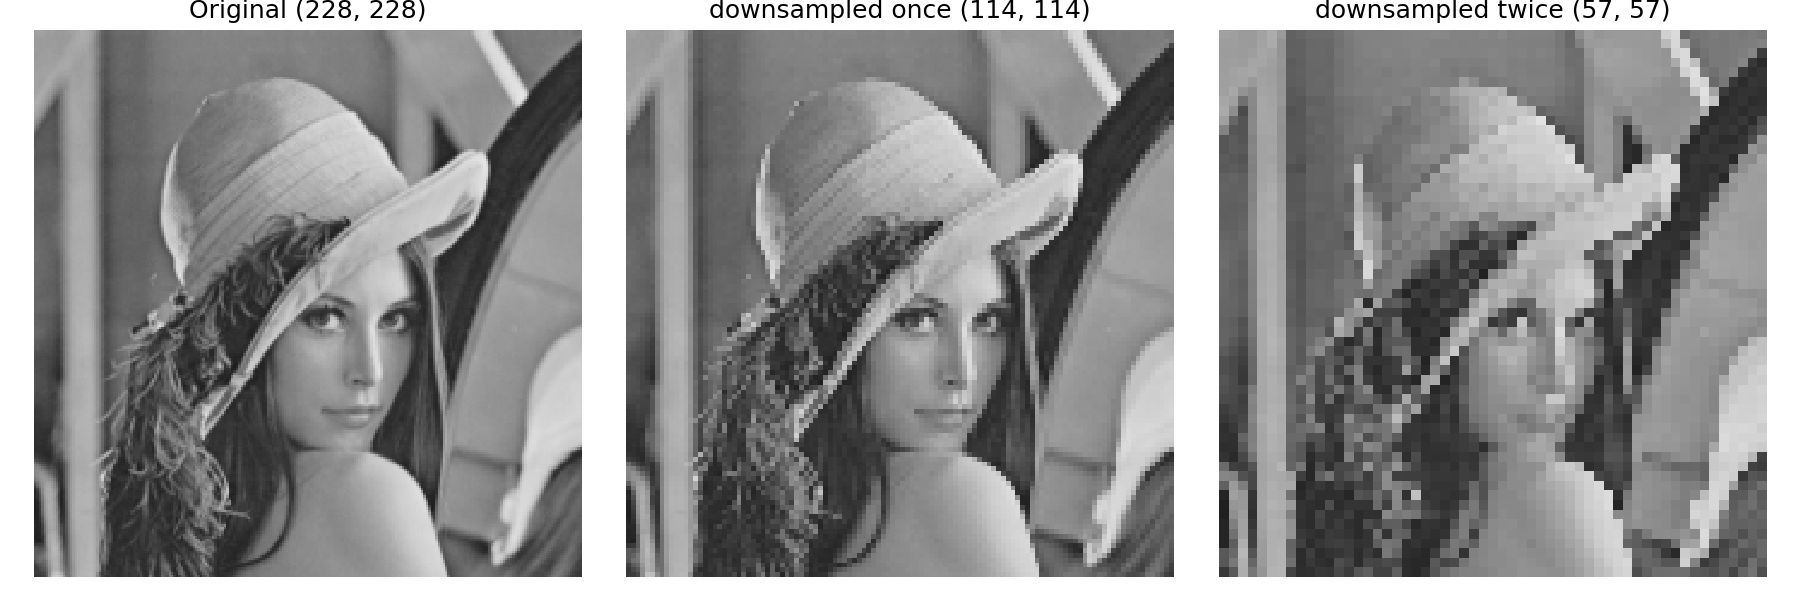
\includegraphics[width=\textwidth]{q1_downsample.png}
  \caption{Original ($228\times228$), downsampled once ($114\times114$) and
  downsampled twice ($57\times57$), displayed at the same size.}
\end{figure}

\textbf{Observation.} As the resolution drops, the images become visibly
blocky: each remaining pixel is drawn as a larger square. Smooth regions such
as the face, shoulder and background wall still look reasonable, because
neighboring pixels there were nearly identical anyway. Fine detail degrades
badly: the diagonal edge of the hat brim turns into a jagged staircase, and
the feathers and the woven texture of the hat lose their structure and turn
into irregular, noisy patterns. At $57 \times 57$, facial features such as the
eyes and mouth are reduced to a few blocks.

\textbf{Why.} Sampling every other pixel keeps only $1/4$ of the samples per
step ($1/16$ after two steps) and assumes each kept pixel represents its
neighborhood. Where the image contains detail finer than the new sampling
spacing, this assumption fails and the sampled values misrepresent the
detail as coarser false patterns. This is \emph{aliasing}: by the Nyquist
theorem, a signal must be sampled at least twice per cycle of its highest
frequency, and halving the sampling rate violates this for the finest
textures. Proper downsampling would first apply a low-pass (smoothing)
filter to remove those frequencies.

\subsection*{Upsampling results}
\begin{figure}[H]
  \centering
  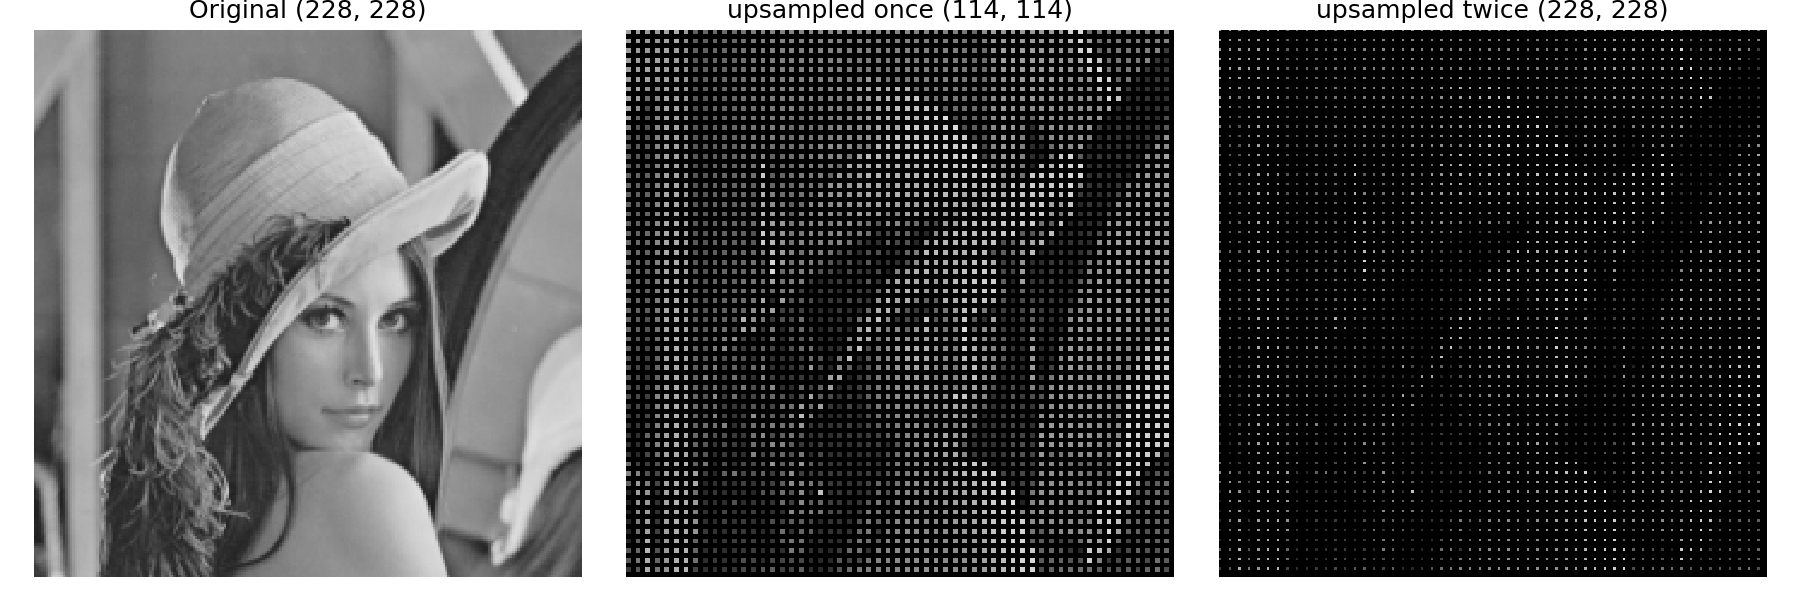
\includegraphics[width=\textwidth]{q1_upsample.png}
  \caption{Original ($228\times228$), upsampled once ($114\times114$) and
  upsampled twice ($228\times228$), starting from the $57\times57$ image.}
\end{figure}

\textbf{Observation.} The upsampled images are covered by a regular grid of
black pixels and are much darker than the original. After one upsampling,
Lena is still recognizable through a fine black mesh. After two, the image
back at the original $228 \times 228$ size consists of sparse isolated bright
dots on a black background and is barely recognizable; it can only be made
out from a distance, where the eye averages the dots together.

\textbf{Why.} Every inserted pixel has value 0. After one upsampling, 3 out
of every 4 pixels are zero, so average brightness drops to roughly $1/4$;
after two, 15 out of every 16 pixels are zero, and brightness drops to
roughly $1/16$. Upsampling restores the image \emph{dimensions} but not the
\emph{information}: the pixels discarded by downsampling are not recovered,
only replaced by empty values. Filling these gaps sensibly requires
interpolation or filtering, which is explored in Problem 3.

\subsection*{Known limitations}
\begin{itemize}
  \item If an image side is not divisible by 4, two halvings followed by two
        doublings do not return exactly to the original size (for example,
        $231 \rightarrow 116 \rightarrow 58 \rightarrow 116 \rightarrow 232$).
        The $228 \times 228$ input avoids this.
  \item No anti-aliasing filter is applied before downsampling, by design of
        the assignment, so aliasing is expected.
\end{itemize}

%==================================================================
\section*{Problem 2: Gaussian Smoothing}

\subsection*{Implementation}
I implemented \texttt{myGaussianSmoothing(I, k, s)} in three steps.

\textbf{1. Kernel.} A $k \times k$ grid of weights is built, where the cell at
horizontal and vertical offset $(x, y)$ from the center gets the raw weight
\[
  G(x, y) = e^{-\frac{x^2 + y^2}{2s^2}}, \qquad x, y \in \{-\lfloor k/2 \rfloor, \dots, \lfloor k/2 \rfloor\}.
\]
All weights are then divided by their sum so the kernel adds up to 1. This
keeps the overall brightness of the image unchanged. (The usual
$\frac{1}{2\pi s^2}$ factor is not needed, since it cancels in this
normalization.) As a check, the $k=3$, $s=1$ kernel is
\[
\begin{bmatrix}
0.075 & 0.124 & 0.075\\
0.124 & 0.204 & 0.124\\
0.075 & 0.124 & 0.075
\end{bmatrix}.
\]

\textbf{2. Padding.} Pixels near the border do not have a full $k \times k$
neighborhood, so the image is padded by $p = \lfloor k/2 \rfloor$ pixels on
every side. Each padded pixel copies the nearest edge pixel (replicate
padding). I chose this over zero padding because zeros would be averaged into
the border and create a dark frame, especially for large $k$.

\textbf{3. Sliding window.} For every pixel of the original image, the
$k \times k$ window around it is taken from the padded image, multiplied
element-wise with the kernel, and summed. That weighted average becomes the
output pixel. The output has the same size as the input, and results are
written to a separate array so every pixel is computed from the original
values. No built-in filtering functions were used; NumPy was used only for
array storage, element-wise multiplication and summing.

Every run starts from the original grayscale image; results are never
smoothed twice.

\subsection*{Experiment 1: varying kernel size ($s = 1$)}
\begin{figure}[H]
  \centering
  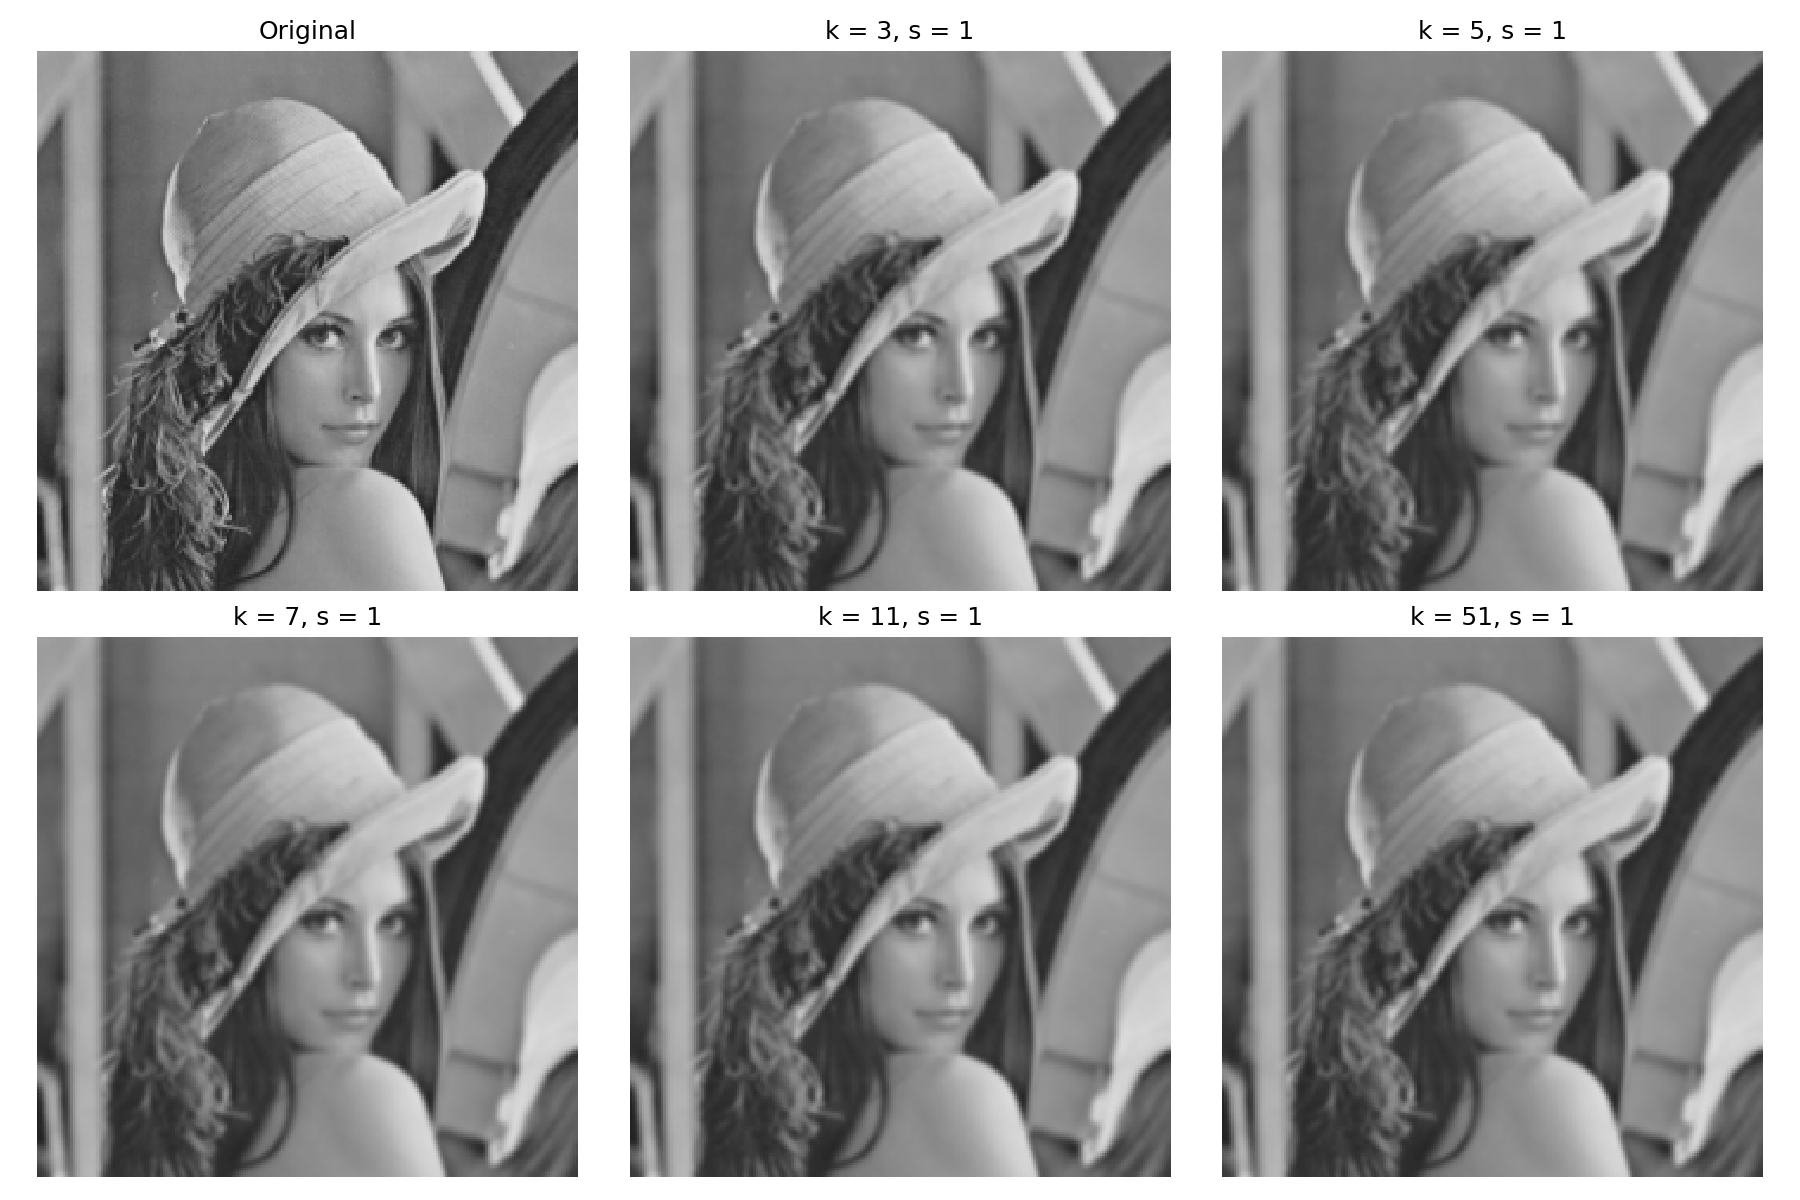
\includegraphics[width=\textwidth]{q2_vary_k.png}
  \caption{Gaussian smoothing with $s = 1$ and $k = 3, 5, 7, 11, 51$.}
\end{figure}

\textbf{Observation.} Going from $k = 3$ to $k = 5$ the image gets
noticeably softer: fine detail such as the feathers, the hat texture and the
eyelashes blurs, and edges like the hat brim become less crisp. From $k = 7$
onward, however, the results look practically identical; $k = 7$, $k = 11$
and $k = 51$ cannot be told apart by eye. The only real difference is run
time, since each output pixel needs $k^2$ multiplications, so $k = 51$ does
about 21 times more work than $k = 11$ for no visible change.

\textbf{Why.} The amount of blur is decided by $s$, not by $k$. With $s = 1$,
the Gaussian weights become negligible beyond about $3s = 3$ pixels from the
center (for example $e^{-4.5} \approx 0.01$ relative to the center at a
distance of 3). A $7 \times 7$ kernel already contains almost all of the
weight, so larger kernels only add near-zero weights at their edges. For
$k = 3$ and $k = 5$ the kernel is too small and cuts off part of the bell
curve, which is why those results are slightly less blurred. In short, $k$
only needs to be large enough to hold the Gaussian (roughly $k \geq 6s + 1$).

\subsection*{Experiment 2: varying $s$ ($k = 11$)}
\begin{figure}[H]
  \centering
  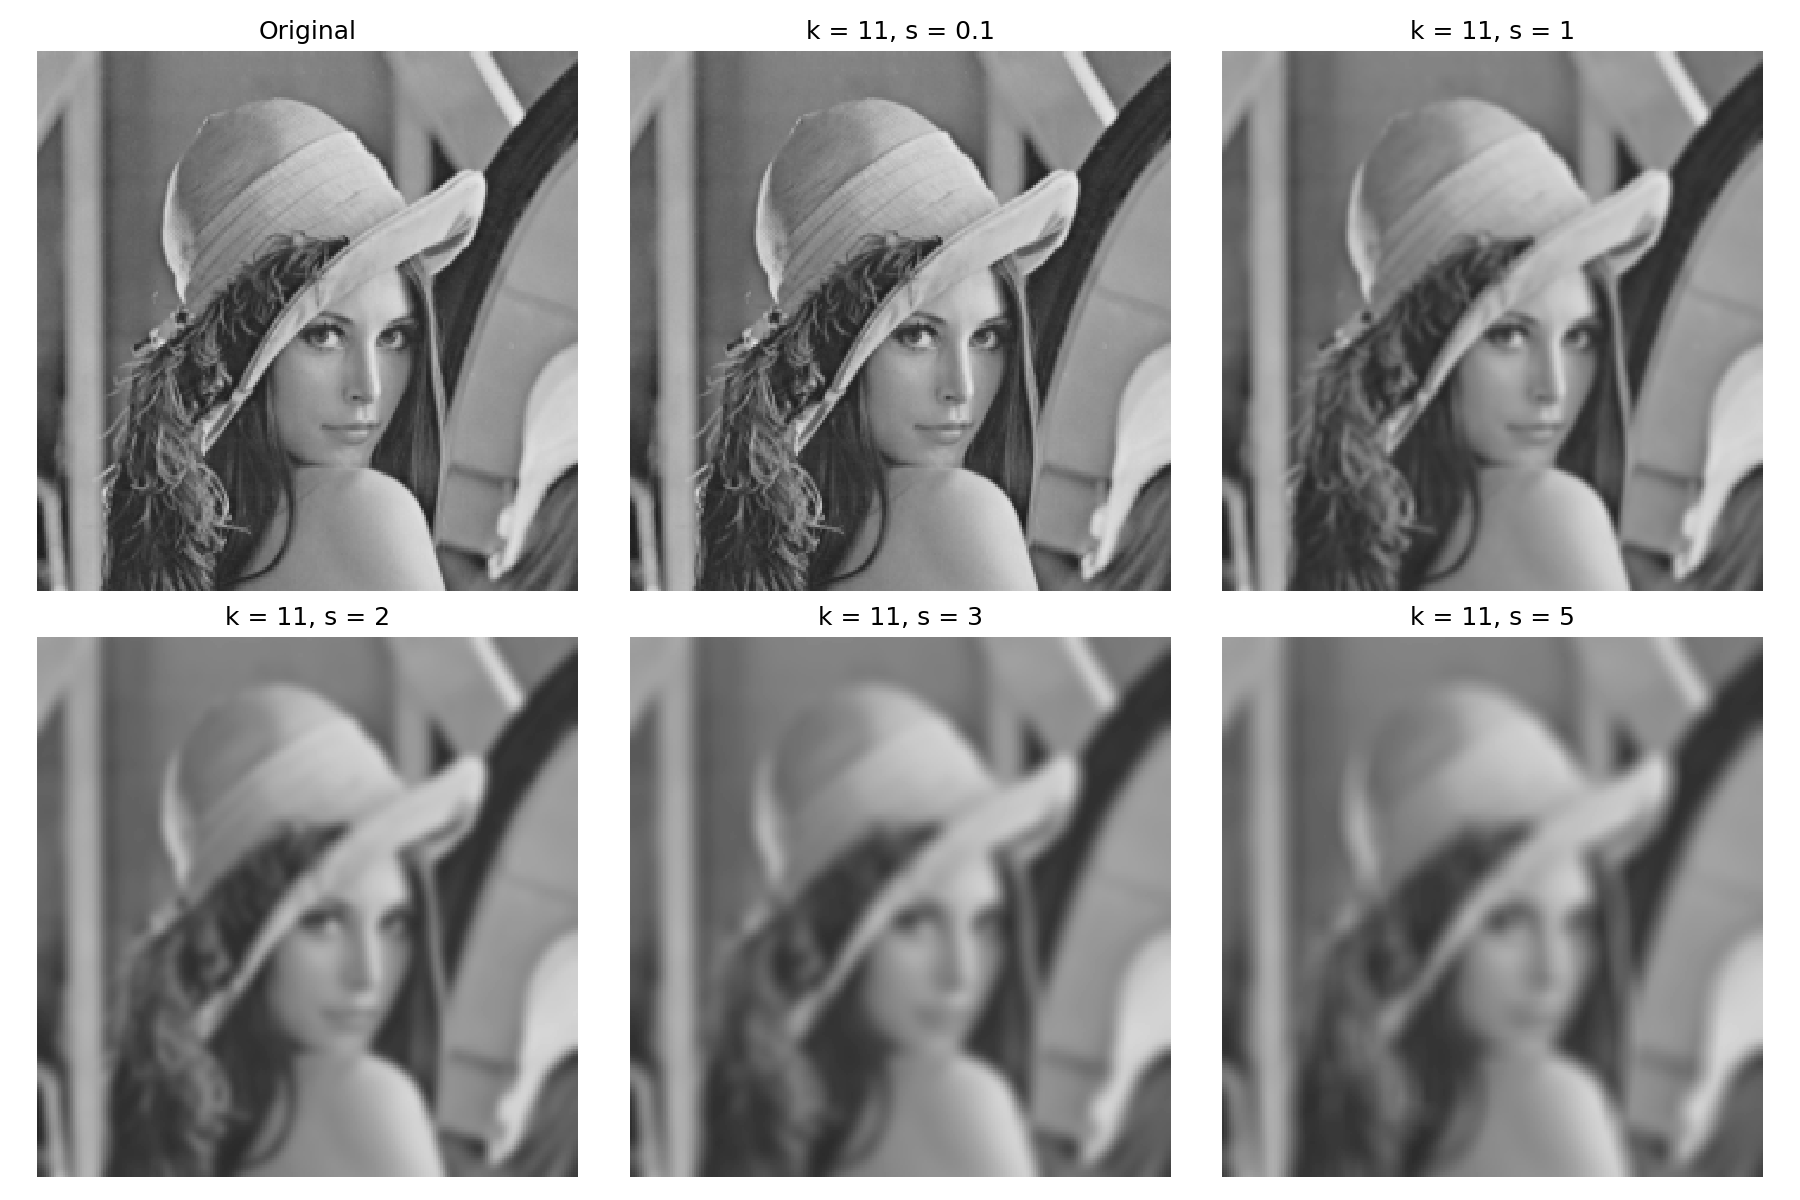
\includegraphics[width=\textwidth]{q2_vary_sigma.png}
  \caption{Gaussian smoothing with $k = 11$ and $s = 0.1, 1, 2, 3, 5$.}
\end{figure}

\textbf{Observation.} With $s = 0.1$ the output looks exactly like the
original. As $s$ increases to 1, 2 and 3, the blur increases steadily: first
fine textures disappear, then facial features and edges soften, and at
$s = 3$ the face and hat are only recognizable by their overall shapes. At
$s = 5$ the image is the most blurred, although the step from $s = 3$ to
$s = 5$ looks smaller than the earlier steps.

\textbf{Why.} $s$ controls how quickly the weights fall off with distance.
At $s = 0.1$ the center weight is essentially 1 and every other weight is
essentially 0, so each pixel is only "averaged" with itself and nothing
changes. Larger $s$ spreads the weight over more distant neighbors, so each
pixel is mixed with a wider area and more high-frequency detail is removed.
At $s = 5$, however, the Gaussian is wider than the $11 \times 11$ window
(which only reaches $\pm 5 = \pm 1s$), so the curve is cut off and the
weights inside the window are nearly flat. The filter then behaves more like
a plain box average of the window, which limits how much extra blur a larger
$s$ can add at this $k$.

\subsection*{Known limitations}
\begin{itemize}
  \item Large kernels are slow: cost grows with $k^2$ per pixel.
  \item When $k$ is small relative to $s$ (e.g.\ $k = 11$, $s = 5$) the
        Gaussian is truncated and the result is not a true Gaussian blur.
  \item Replicate padding repeats edge pixels, so a few pixels along the
        border are slightly biased toward the edge values.
\end{itemize}


\section*{Problem 3: Image Filtering}

\subsection*{Implementation}
Starting from the $57 \times 57$ image obtained in Problem 1 (downsampling
twice), I repeated the upsampling from Problem 1 but applied a filter after
\emph{every} upsampling step, so each filtered result is the input to the
next upsampling:
\[
57 \xrightarrow{\text{up}} 114 \xrightarrow{\text{filter}} 114
   \xrightarrow{\text{up}} 228 \xrightarrow{\text{filter}} 228 .
\]
This was done twice, once with each filter, both starting from the same
upsampled data.

\textbf{Gaussian filter.} My Gaussian smoothing function from
Problem 2 (named \texttt{gaussianSmoothing} in this script) with $k = 11$ and $\sigma = 1$, as specified.

\textbf{Median filter.} I implemented my own median filter using the same
structure as the Gaussian filter: the image is padded by replicating edge
pixels, and for every pixel the $k \times k$ window around it is taken. Instead
of a weighted sum, the window values are flattened into a list, sorted, and the
middle element (index $\lfloor k^2/2 \rfloor$) becomes the output pixel. The
median filter has no weights and therefore no $\sigma$. Since the question does
not specify a size, I used the standard $3 \times 3$ window ($k = 3$). As a
check, the filter turns
$\begin{bmatrix} 5 & 5 & 5\\ 5 & 999 & 5\\ 5 & 5 & 5 \end{bmatrix}$
into a matrix of all 5s, removing the outlier.

\subsection*{Results: Gaussian filtering}
\begin{figure}[H]
  \centering
  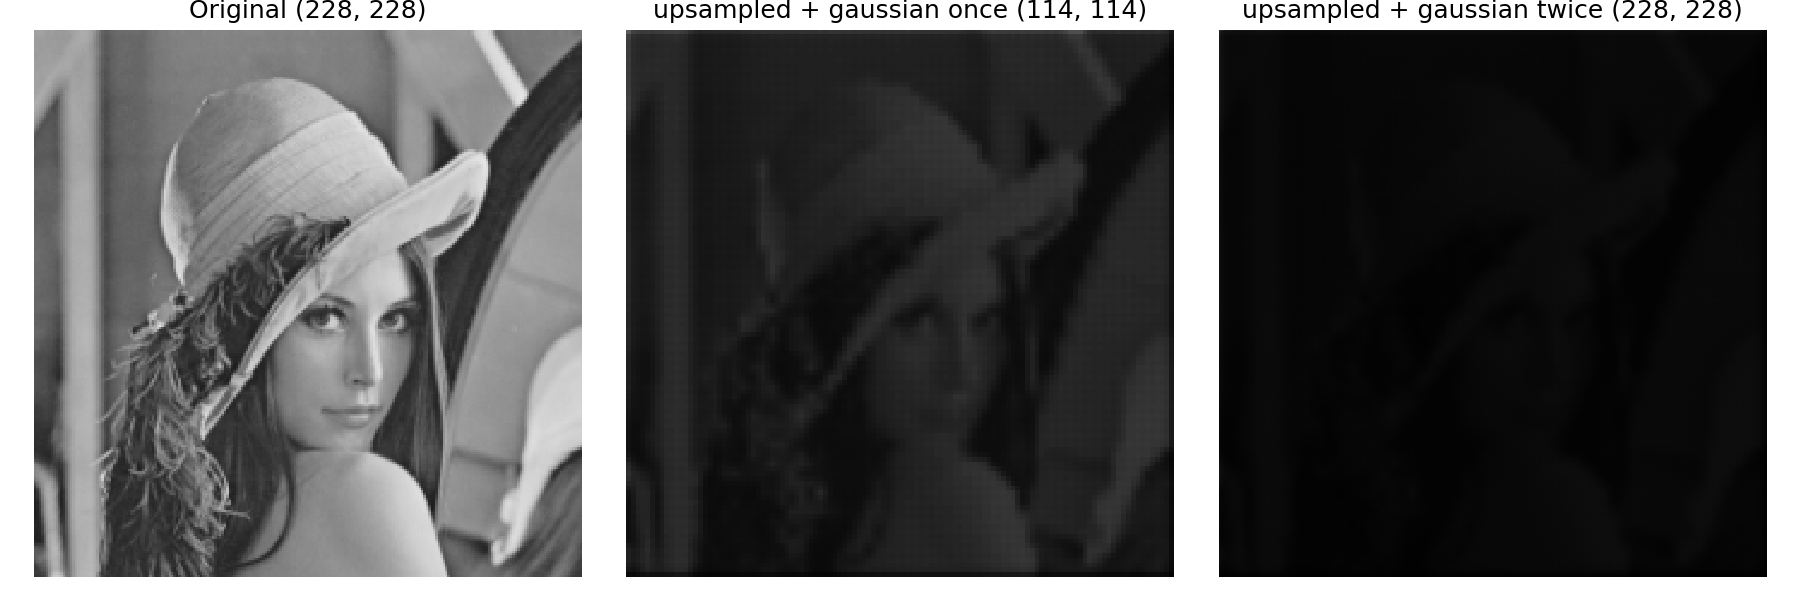
\includegraphics[width=\textwidth]{q3_upsample_gaussian.png}
  \caption{Upsampling with Gaussian smoothing ($k = 11$, $\sigma = 1$) after
  each upsampling step.}
\end{figure}

\textbf{Did it get better?} Partly. Compared with Problem 1, the regular grid
of black pixels is gone and the image is smooth and recognizable again. A very
faint leftover dot texture is still visible after the first step. However, the
results are blurry, and they are much darker than the original: roughly
$1/4$ of the original brightness after the first step and $1/16$ after the
second, so the final image is close to black.

\textbf{Why.} The Gaussian spreads every real pixel into the empty positions
around it, which fills the gaps. But its weights sum to 1, so each output is an
average that includes the inserted zeros. After one upsampling, 3 of every 4
pixels are zero, so the average brightness drops to about $1/4$; the second
step repeats this, giving about $1/16$. The structure is preserved, only scaled
down: multiplying the final result by 16 restores the original brightness and
shows a smooth, blurred version of the image. The blur itself is unavoidable,
since the detail removed by downsampling cannot be recovered. The faint
leftover texture appears because $\sigma = 1$ is only just wide enough to fill
gaps 2 pixels apart evenly.

\subsection*{Results: median filtering}
\begin{figure}[H]
  \centering
  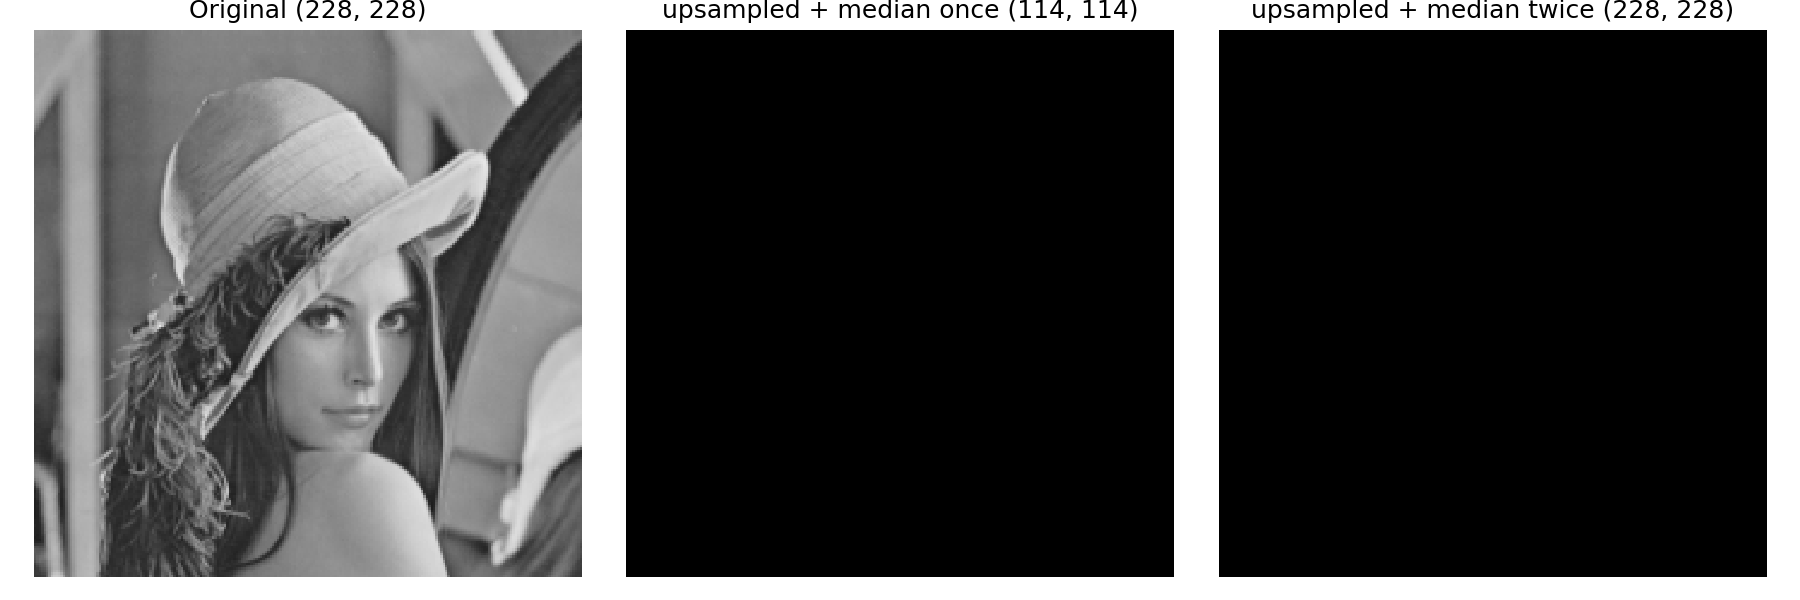
\includegraphics[width=\textwidth]{q3_upsample_median.png}
  \caption{Upsampling with $3 \times 3$ median filtering after each
  upsampling step.}
\end{figure}

\textbf{Did it improve the result?} No. Both results are completely black;
the largest value in either image is exactly 0. The median filter removed the
image entirely.

\textbf{Why.} After upsampling, real pixels sit only at even positions. Any
$3 \times 3$ window therefore contains 1, 2 or 4 real pixels, and at least 5
zeros:
\[
\begin{bmatrix} 0&0&0\\ 0&R&0\\ 0&0&0 \end{bmatrix}
\qquad
\begin{bmatrix} 0&0&0\\ R&0&R\\ 0&0&0 \end{bmatrix}
\qquad
\begin{bmatrix} R&0&R\\ 0&0&0\\ R&0&R \end{bmatrix}
\]
After sorting the 9 values, the middle (5th) value is always 0. The median's
strength is ignoring a minority of extreme values as outliers, but here the
real image pixels \emph{are} the minority, so the filter treats the image
itself as noise and discards it. The second step starts from an all-black
image and stays black. A larger window does not help, because real pixels
remain at most about a quarter of any window.

\subsection*{Which filtering is better?}
Gaussian filtering is clearly better here. It fills the gaps with a weighted
blend of the nearby real pixels, so the image survives, although blurred and
darkened. Median filtering fails completely. This does not mean the median
filter is a bad filter; it works well when the corrupted values are rare
(for example, salt-and-pepper noise), but in upsampled data the inserted zeros
are the majority.

\subsection*{Known limitations}
\begin{itemize}
  \item The Gaussian results are darkened by averaging with the inserted
        zeros; no brightness correction is applied in the main results.
  \item A thin darker line appears along the right and bottom edges of the
        Gaussian results: the last row and column of each upsampled image are
        zeros, and edge-replicate padding copies them outward.
  \item Neither filter recovers the fine detail lost during downsampling.
\end{itemize}


\section*{Problem 4: Noise}

\subsection*{Implementation}
\textbf{Gaussian noise.} Using the original grayscale image $I$, I generated
one random value per pixel, $r \sim N(0, 0.1)$, and formed
$I_{\text{noisy}}(x, y) = I(x, y) + r$. I interpreted $0.1$ as the standard
deviation. The result was clipped to $[0, 1]$ so it remains a valid image. The
random generator was seeded so the noise, and therefore every figure, is
reproducible.

\textbf{Filtering.} The noisy image was filtered with my Gaussian smoothing
from Problem 2 using $k = 7$ and $\sigma = 1$ (a $7 \times 7$ window holds
almost all of a $\sigma = 1$ Gaussian, as found in Problem 2), and with my
$3 \times 3$ median filter from Problem 3. Each filter was applied directly to
the noisy image.

\textbf{Salt noise.} Using the \emph{same} noise values $r$, I set the noise to
1 where $r > 0.2$ and 0 otherwise, and added this to the original image,
again clipping to $[0, 1]$. With a standard deviation of 0.1, $r > 0.2$ happens
for about 2.3\% of pixels, so roughly 2\% of the pixels become pure white and
the rest are unchanged. Because only large \emph{positive} values pass the
threshold, this produces white dots only (salt), with no black dots (pepper).
The same two filters with the same settings were then applied.

\subsection*{Results}
\begin{figure}[H]
  \centering
  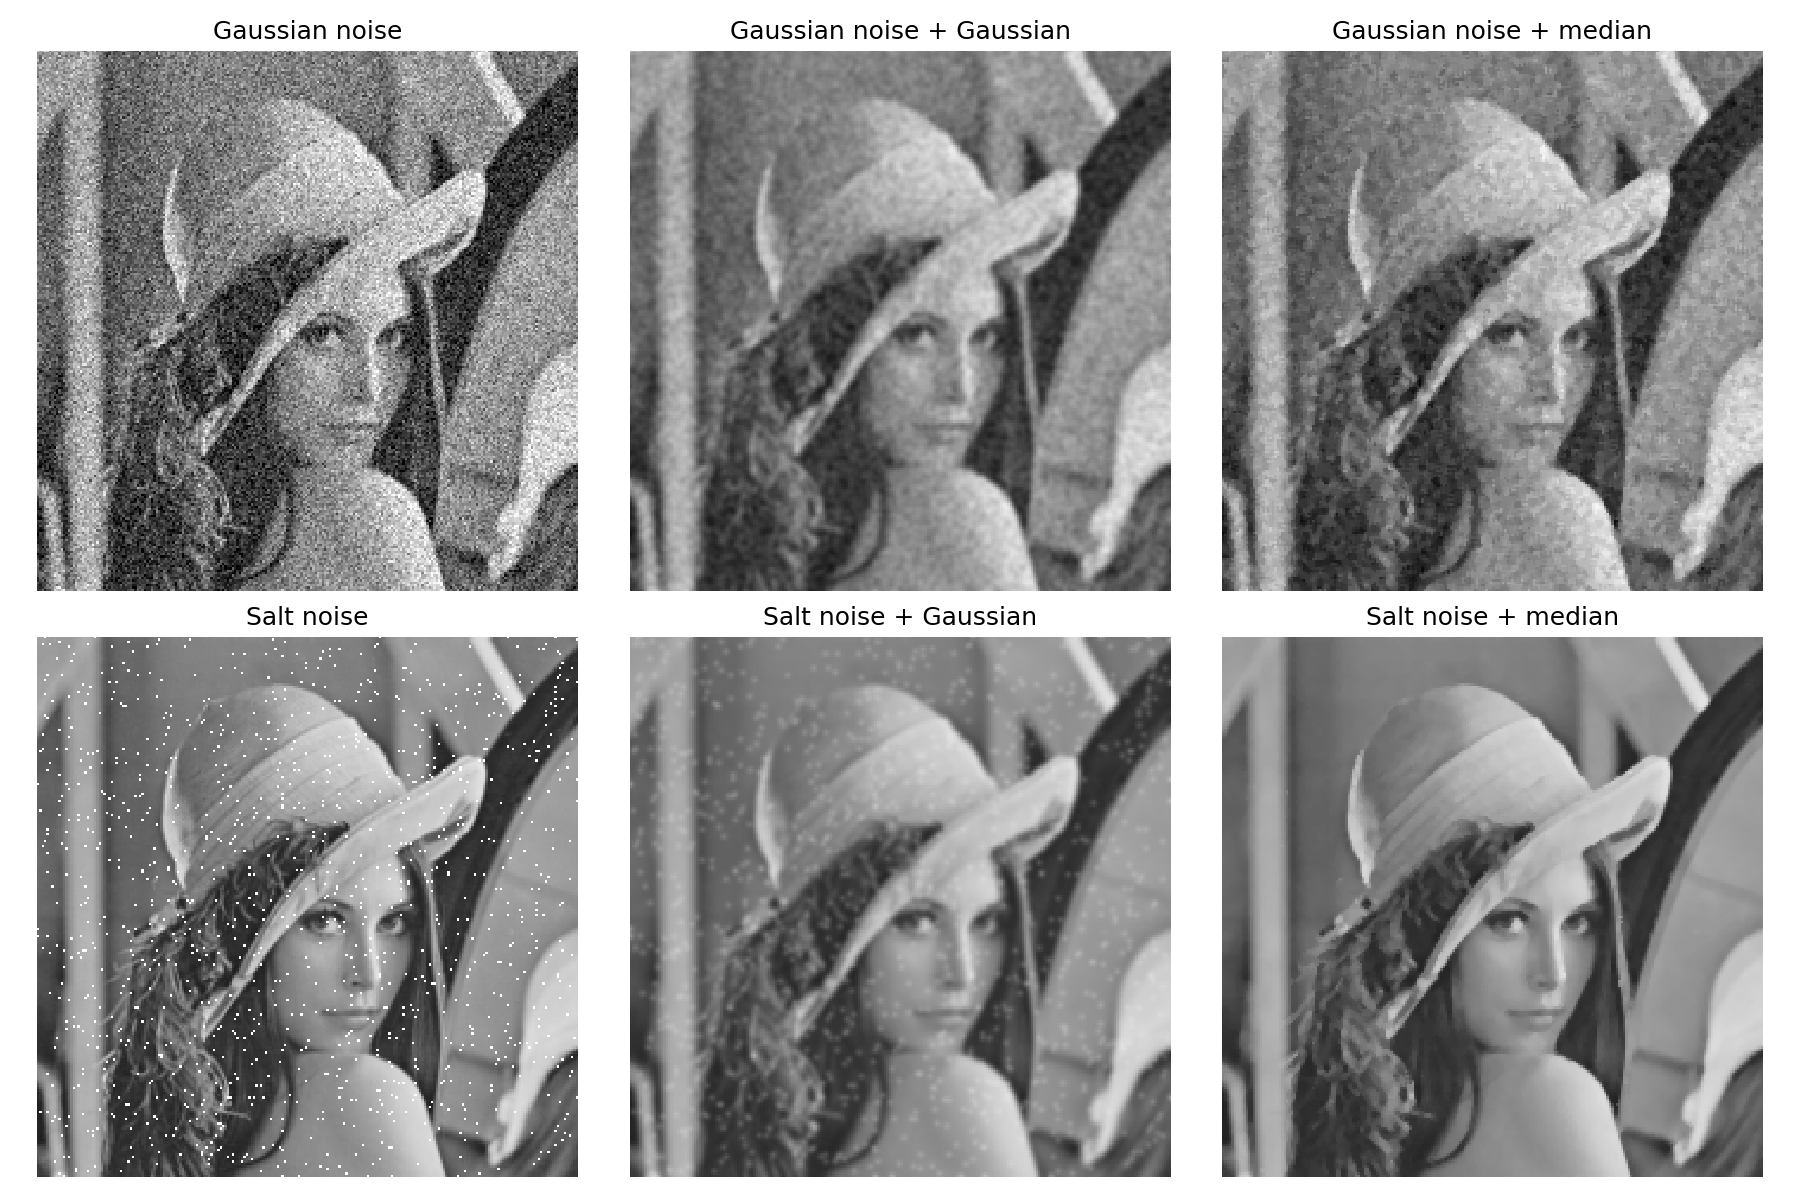
\includegraphics[width=\textwidth]{q4_noise.png}
  \caption{Top row: Gaussian noise, then Gaussian smoothing ($k = 7$,
  $\sigma = 1$) and $3 \times 3$ median filtering. Bottom row: salt noise, then
  the same two filters.}
\end{figure}

\textbf{Gaussian noise: how does it look?} The image is grainy everywhere, like
static. Every pixel is slightly brighter or darker than it should be, but the
content is still clearly recognizable.

\textbf{Gaussian smoothing: did it improve?} Yes, clearly. The grain is mostly
gone. Because the noise values are random and centered on zero, averaging a
pixel with its neighbors makes the positive and negative errors cancel out. The
cost is some blur: edges and fine texture become softer.

\textbf{Median filtering on Gaussian noise.} It also improves the image and
keeps edges somewhat sharper, but a blotchy texture remains and the result is
less clean than the Gaussian. With Gaussian noise every pixel is a little wrong,
so there is no ``clean majority'' in the window for the median to pick; it just
selects one of the noisy values. Averaging uses all the values and cancels
noise more effectively.

\textbf{Salt noise: Gaussian smoothing.} The white dots are not removed. Each
dot is averaged with its neighbors, so it is spread into a fainter gray smudge,
and the whole image is blurred as well. The corruption is diluted, not
eliminated.

\textbf{Salt noise: median filtering.} This gives the best result in the whole
figure: the white dots disappear almost completely and the image stays sharp.
A white dot is typically only 1 of the 9 values in a $3 \times 3$ window, so
after sorting it sits at the end of the list and the middle value is an
ordinary, uncorrupted pixel. Since most pixels are untouched, edges are also
preserved.

\subsection*{Discussion}
The two filters suit different kinds of noise. Gaussian smoothing works best
when \emph{every} pixel is slightly corrupted, because averaging cancels small
random errors. Median filtering works best when \emph{a few} pixels are
completely corrupted, because the median ignores a minority of extreme values
(outliers) instead of averaging them in.

This also explains the median filter's failure in Problem 3. There, the
inserted zeros were the \emph{majority} of each window and the real pixels were
the minority, so the median discarded the image. Here the salt dots are the
minority, so the median discards exactly the noise.

\subsection*{Known limitations}
\begin{itemize}
  \item $N(0, 0.1)$ was interpreted as standard deviation 0.1. If it meant
        variance 0.1 (standard deviation about 0.32), the noise would be much
        stronger and about 26\% of pixels would become salt, which would make
        the median filter less effective.
  \item Clipping to $[0, 1]$ slightly changes the noise near black and white
        regions.
  \item A single, fixed random seed was used; other seeds give visually
        identical conclusions but different individual noise pixels.
\end{itemize}


\section*{Problem 5: Sobel Filters}

\subsection*{Implementation}
I implemented \texttt{mySobelFilter(I)}, which returns the edge magnitude and
orientation for every pixel. It uses the two $3 \times 3$ Sobel kernels
\[
G_x = \begin{bmatrix} -1 & 0 & 1\\ -2 & 0 & 2\\ -1 & 0 & 1 \end{bmatrix},
\qquad
G_y = \begin{bmatrix} -1 & -2 & -1\\ 0 & 0 & 0\\ 1 & 2 & 1 \end{bmatrix}.
\]
$G_x$ subtracts the left column of a pixel's neighborhood from the right column,
measuring how brightness changes from left to right; $G_y$ does the same from
top to bottom. The larger weight in the middle row/column gives the pixels
closest to the center more influence, which adds a little smoothing. Each kernel
is applied with the same sliding-window function used for Gaussian smoothing
(edge-replicate padding, element-wise multiply and sum), giving the gradients
$g_x$ and $g_y$. Then
\[
\text{mag} = \sqrt{g_x^2 + g_y^2}, \qquad \text{ori} = \operatorname{arctan2}(g_y, g_x).
\]
The magnitude is the edge strength; the orientation is the direction in which
brightness increases most, in $[-\pi, \pi]$. \texttt{arctan2} was used instead of
$\arctan(g_y/g_x)$ so the full range of directions is kept and division by zero
is avoided.

\textbf{Normalization to $[0,1]$.} The magnitude is divided by its maximum. The
orientation is mapped with $(\text{ori} + \pi)/(2\pi)$. For display, $g_x$ and
$g_y$, which can be negative, are min--max normalized, so mid-gray means no
change, darker means brightness decreases and brighter means it increases.

\textbf{Color visualization.} An HSV image was built with hue $=$ orientation,
saturation $=$ magnitude and value $=$ magnitude, and converted to RGB for
display using matplotlib's \texttt{hsv\_to\_rgb} (used only for this color
conversion; the Sobel filter itself uses no built-in functions).

\subsection*{Results}
\begin{figure}[H]
  \centering
  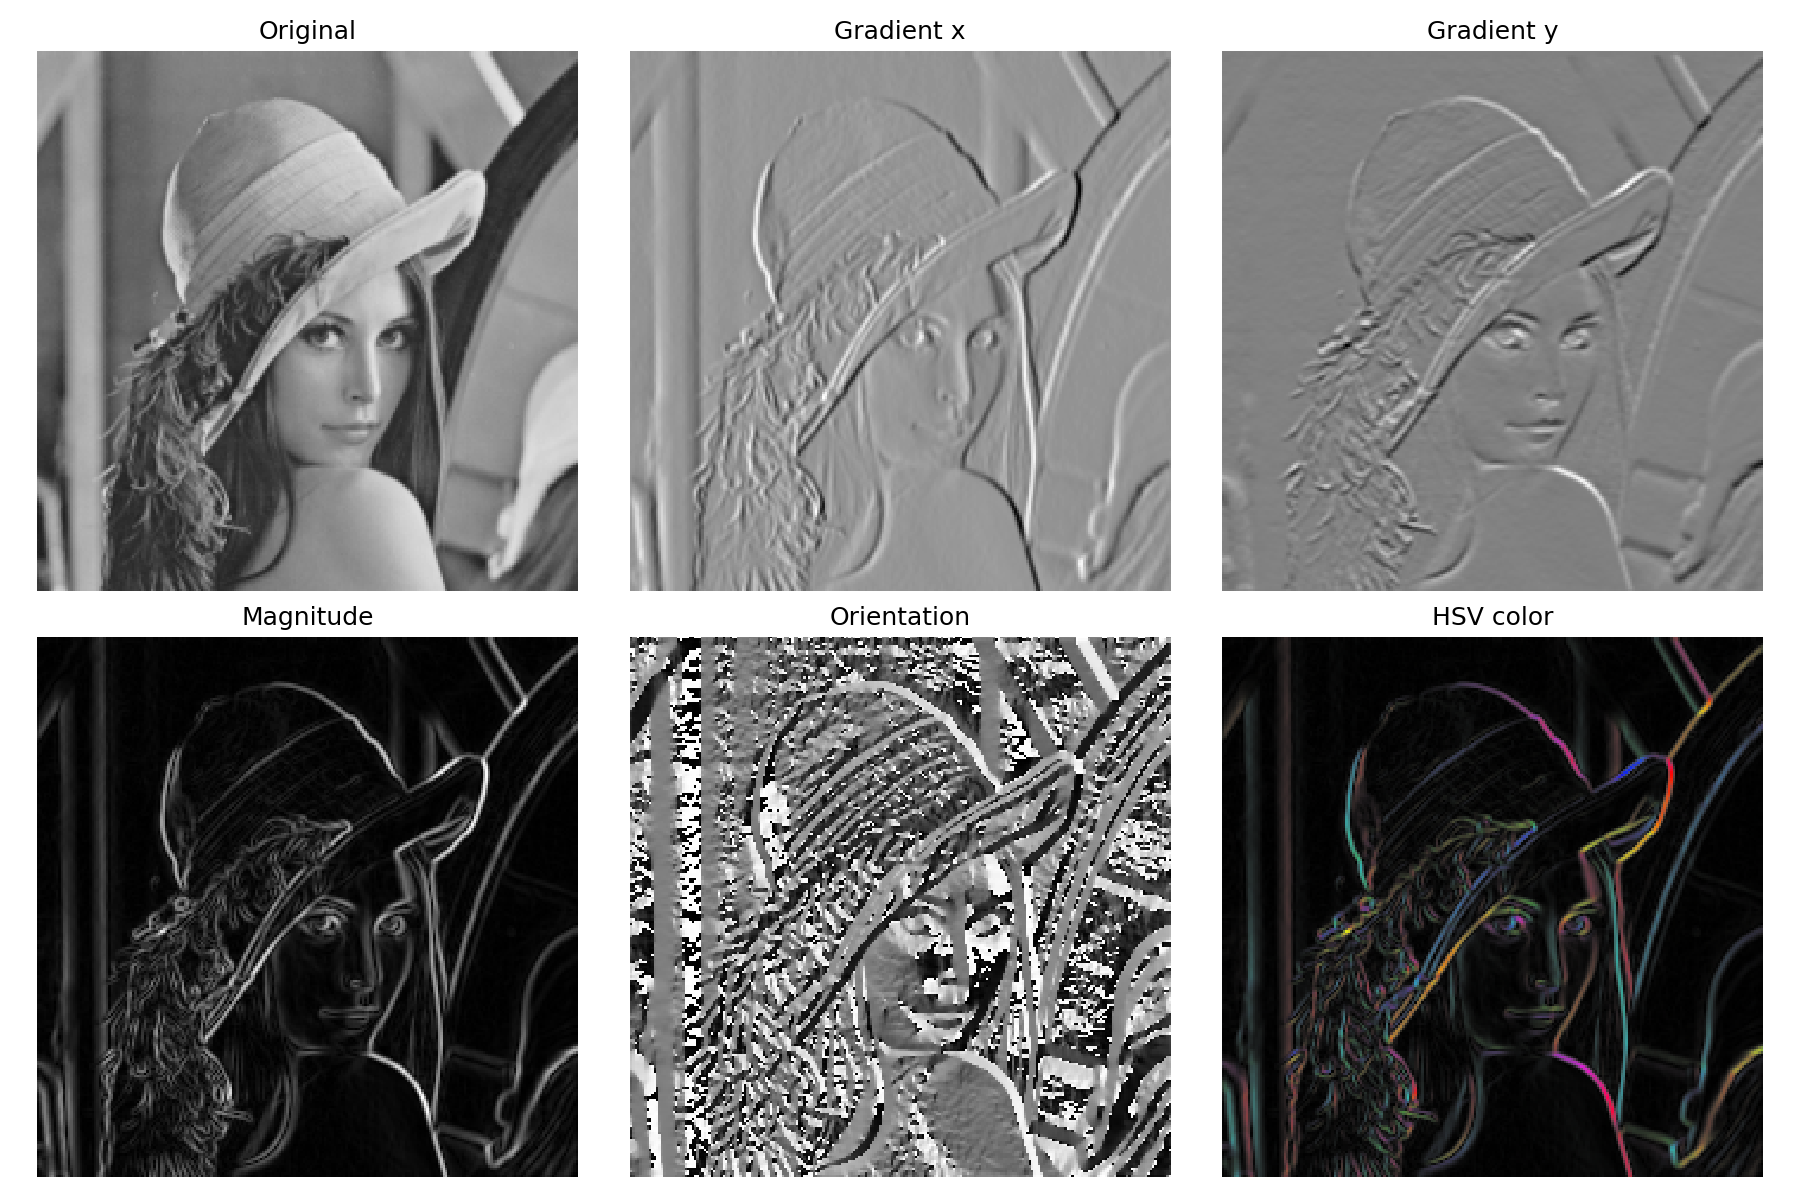
\includegraphics[width=\textwidth]{q5_sobel.png}
  \caption{Original, normalized $x$ and $y$ gradients, normalized magnitude,
  normalized orientation, and the HSV visualization.}
\end{figure}

\textbf{Gradients.} Both gradient images look like an embossed version of Lena.
The $x$ gradient responds mainly to vertical edges (the sides of the hat, the
hair strands, the edge of the shoulder), while the $y$ gradient responds mainly
to horizontal edges (the top of the hat brim, the eyes, the lips). Flat regions
are mid-gray in both, meaning no change.

\textbf{Magnitude.} The magnitude image is black in smooth regions such as the
background, cheek and shoulder, and bright along object boundaries. The
strongest responses are on high-contrast boundaries like the hat brim and the
outline of the shoulder, while the feathers and hair produce many weaker,
densely packed edges. This matches the idea that an edge is a place of rapid
intensity change.

\textbf{Orientation.} On its own, the orientation image is hard to read. Along
real edges it is consistent, but in flat regions it looks like random noise,
because there $g_x$ and $g_y$ are both close to zero and their angle is
determined by tiny intensity fluctuations. There are also sharp jumps from black
to white, which are not real edges: angles just below $+\pi$ and just above
$-\pi$ point in almost the same direction but map to opposite ends of $[0,1]$.

\textbf{HSV visualization.} Using magnitude for saturation and value solves this.
Flat regions become black, hiding their meaningless orientations, and only real
edges are visible, colored by their direction. Edges with the same orientation
share a color along their length, such as the long boundary of the hat brim, and
the color changes gradually as an edge curves. The two sides of a thin
structure often appear in different colors, since the brightness increases in
opposite directions on each side. The hue wraps around the color wheel, so the
angle jump that looked like a black-to-white break in the grayscale orientation
image appears as a smooth red-to-red transition here. The result resembles the
color-coded Sobel example from the lecture.

\subsection*{Known limitations}
\begin{itemize}
  \item No smoothing is applied before the Sobel filter, so weak texture and
        noise also produce small responses; smoothing first (as discussed in
        lecture) would reduce these at the cost of some edge sharpness.
  \item Orientation is unreliable where the magnitude is near zero.
  \item Magnitude is normalized by the maximum of this image, so values are
        relative to the strongest edge rather than absolute.
\end{itemize}


\end{document}